% !TEX root = ../dg.tex

\section{The Exponential Map}
\label{sec:exponential map}

In classifying Lie groups (especially compact Lie groups), it turns out to be particularly helpful to understand the abelian subgroups, and especially the maximal abelian subgroups (so-called \emph{maximal tori}). The simplest abelian subgroups are called one-parameter subgroups:

\begin{definition}\label{def:one-parameter subgroups}
	A homomorphism $\phi \from \R \to G$ with closed image (or sometimes the image of such a homomorphism) is called a \emph{one-parameter subgroup} of $G$.
\end{definition}

\begin{example}
	The map $\phi \from \R \to U(1) \times U(1)$ defined by $\phi(t) = \left(e^{it}, e^{i \sqrt{2}t}\right)$ is \emph{not} a one-parameter subgroup because its image is dense, and hence not closed.
\end{example}

\begin{example}\label{ex:one-parameter subgroup of SO(3)}
	Define $\phi \from \R \to \SO(3)$ by
	\[
		\phi(t) = \begin{bmatrix} \cos t & - \sin t & 0 \\ \sin t & \cos t & 0 \\ 0 & 0 & 1 \end{bmatrix}.
	\]
	Then $\phi$ is a one-parameter subgroup of $\SO(3)$, which corresponds to rotations around the $z$-axis. Of course, $\phi$ is periodic and in fact descends to an injective homomorphism $\SO(2) \to \SO(3)$ (where $\SO(2)$ is diffeomorphic to the circle).
	
	Notice that 
	\[
		\phi'(0) = \begin{bmatrix} 0 & -1 & 0 \\ 1 & 0 & 0 \\ 0 & 0 & 0 \end{bmatrix} \in \mathfrak{so}(3);
	\]
	in fact, this is one of the basis elements we found in the proof of \Cref{prop:accidental isomorphisms}. Indeed, $\phi(t) = \gamma_3(t)$ from HW 3, Problem 2.
	
	In that notation, we also have
	\[
		\gamma_1(t) = \begin{bmatrix} 1 & 0 & 0 \\ 0 & \cos t & - \sin t \\ 0 & \sin t & \cos t\end{bmatrix} \quad \text{and} \quad \gamma_2(t) = \begin{bmatrix} \cos t & 0 &  \sin t \\ 0 & 1 & 0 \\ -\sin t & 0 & \cos t \end{bmatrix},
	\]
	and these also define one-parameter subgroups. More generally, if $a,b,c \in \R$, then
	\[
		\gamma(t) := \gamma_1(at) \gamma_2(bt) \gamma_3(ct)
	\]
	defines a one-parameter subgroup with
	\[
		\gamma'(0) = a\gamma_1'(0) \gamma_2(0) \gamma_3(0) + b\gamma_1(0) \gamma_2'(0) \gamma_3(0) + c \gamma_1(0) \gamma_2(0) \gamma_3'(0) = \begin{bmatrix} 0 & -c & b \\ c & 0 & -a \\ -b & a & 0 \end{bmatrix},
	\]
	so we see that every element of $\mathfrak{so}(3)$ determines a one-parameter subgroup.
\end{example}

This is a general phenomenon: if $G$ is a Lie group and $X \in \mathfrak{g}$, then the map $\lambda \frac{d}{dr} \mapsto \lambda X$ defines a homomorphism from the Lie algebra of $\R$ into $\mathfrak{g}$. Since $\R$ is simply-connected, \Cref{thm:Lie group Lie algebra correspondence} guarantees there exists a unique one-parameter subgroup $\phi_X \from \R \to G$ so that $d\phi_X\left(\lambda \frac{d}{dr} \right) = \lambda X$.

\begin{definition}\label{def:exponential map}
	Define the \emph{exponential map} $\exp \from \mathfrak{g} \to G$ by $\exp(X) = \phi_X(1)$.
\end{definition}

\begin{example}
	Let $G = \U(1)$, the unit complex numbers. We can identify $\mathfrak{u}(1)$ with the tangent space at the identity $T_1 \U(1)$, which is visually just a copy of the imaginary axis, as we see in \Cref{fig:circletangent}.
	
	\begin{figure}[htbp]
		\centering
			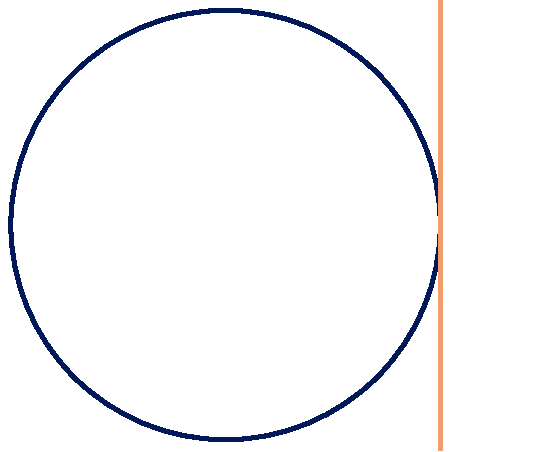
\includegraphics[height=1.5in]{circletangent}
		\caption{The tangent space at 1 to the unit circle.}
		\alttext{A circle together with the tangent line to the rightmost point.}
		\label{fig:circletangent}
	\end{figure}
	
	We can make the identification $\mathfrak{u}(1) \cong i \R$. Let $X = i a \in \mathfrak{u}(1)$ and define the map $\phi_X \from \R \to \U(1)$ by $\phi_X(r) = e^{rX} = e^{i a r}$. Since $\phi_X'(0) = ia = X$, this is the one-parameter subgroup guaranteed by \Cref{thm:Lie group Lie algebra correspondence}, and so by definition
	\[
		\exp(X) = \phi_X(1) = e^X = e^{ia}.
	\]
	
	\ifplastex
	\begin{figure}[htbp]
		\centering
			\includegraphics[height=2in]{wrap.gif}
		\caption{An animation of the exponential map on the unit circle. See also this \href{https://community.wolfram.com/groups/-/m/t/2148879}{more artistic version}.}
		\alttext{The tangent line from the previous figure is wrapped around the circle in a continuous fashion.}
		\label{fig:wrap}
	\end{figure}
	\fi
	
	This helps explain the source of the name: the exponential map on $\U(1)$ is just the usual exponential map from complex analysis.
\end{example}

More generally, suppose $A \in \Mat_{n\times n}(\R) \cong \mathfrak{gl}_n(\R)$ and define $\gamma(t) = e^{tA}$, where the matrix exponential is defined by the Taylor series
\[
	e^M := I + M + + \frac{1}{2!} M^2 + \frac{1}{3!} M^3 + \dots
\]
(which turns out to converge everywhere, just like the usual Taylor series for the single variable exponential). Then
\[
	\gamma'(0) = \left. \frac{d}{dt} \right|_{t=0} e^{tA} = \left. A e^{tA} \right|_{t=0} = A,
\]
so $\gamma(t) = \phi_X(t)$ and hence $\exp(A) = \gamma(1) = e^A$. In other words, the exponential map on matrix groups is always just the matrix exponential.

\begin{example}
	Let 
	\[
		A = \begin{bmatrix} 0 & -1 & 0 \\ 1 & 0 & 0 \\ 0 & 0 & 0 \end{bmatrix} \in \mathfrak{so}(3).
	\]
	By uniqueness, we know that 
	\[
		e^{tA} = \exp(tA) = \begin{bmatrix} \cos t & -\sin t & 0 \\ \sin t & \cos t & 0 \\ 0 & 0 & 1 \end{bmatrix},
	\]
	our one-parameter subgroup from \Cref{ex:one-parameter subgroup of SO(3)}. But we can also prove this directly by computing powers of $A$:
	\[
		A =  \begin{bmatrix} 0 & -1 & 0 \\ 1 & 0 & 0 \\ 0 & 0 & 0 \end{bmatrix}, \quad A^2 =  \begin{bmatrix} -1 & 0 & 0 \\ 0 & -1 & 0 \\ 0 & 0 & 0 \end{bmatrix}, \quad A^3 =  \begin{bmatrix} 0 & 1 & 0 \\ -1 & 0 & 0 \\ 0 & 0 & 0 \end{bmatrix}, \quad A^4 =  \begin{bmatrix} 1 & 0 & 0 \\ 0 & 1 & 0 \\ 0 & 0 & 0 \end{bmatrix}.
	\]
	After this, the powers repeat, so we see that
	\[
		e^{tA} = I + tA + \frac{1}{2!} (tA)^2 + \dots = \begin{bmatrix} 1 - \frac{t^2}{2!} + \frac{t^4}{4!} & -t + \frac{t^3}{3!} - \frac{t^5}{5!} & 0 \\ t - \frac{t^3}{3!} + \frac{t^5}{5!} & 1 - \frac{t^2}{2!} + \frac{t^4}{4!} & 0 \\ 0 & 0 & 0 \end{bmatrix} = \begin{bmatrix} \cos t & -\sin t & 0 \\ \sin t & \cos t & 0 \\ 0 & 0 & 0 \end{bmatrix}
	\]
	using the Taylor series for sine and cosine.
\end{example}

\begin{example}\label{ex:general one-parameter subgroup of SO(3)}
	More generally, consider
	\[
		X = \begin{bmatrix} 0 & -z & y \\ z & 0 & -x \\ -y & x & 0 \end{bmatrix} \in \mathfrak{so}(3),
	\]
	where $x^2 + y^2 + z^2 = 1$. That is, $v = (x,y,z) \in \R^3$ is a unit vector and $X = F(v)$ in the notation of \Cref{ex:so3 Lie algebra}. 
	
	The characteristic polynomial of $X$ is
	\[
		P(\lambda) = \det(\lambda I - X) = \det \begin{bmatrix} \lambda & z & -y \\ -z & \lambda & x \\ y & -x & \lambda \end{bmatrix} = \lambda^3 + \lambda(x^2 + y^2 + z^2) = \lambda^3 + \lambda,
	\]
	so the Cayley–Hamilton theorem implies $0 = P(X) = X^3 + X$, so $X^3 = -X$, and hence
	\begin{align*}
		\exp(tX) & = I + tX + \frac{1}{2!} (tX)^2 + \frac{1}{3!} (tX)^3 + \dots \\
		& = I + tX + \frac{t^2}{2!} X^2 - \frac{t^3}{3!} X - \frac{t^4}{4!} X^2 + \dots \\
		& = I + \left(t - \frac{t^3}{3!} + \dots \right)X + \left(\frac{t^2}{2!} - \frac{t^4}{4!} + \dots \right)X^2 \\
		& = I + (\sin t) X + (1-\cos t)X^2.
	\end{align*}
	
	Therefore, for $u = (a,b,c) \in \R^3$, we have that
	\[
		Xu = \begin{bmatrix} 0 & -z & y \\ z & 0 & -x \\ -y & x & 0 \end{bmatrix} \begin{bmatrix} a \\ b \\ c \end{bmatrix} = \begin{bmatrix} -bz + cy \\ az-cx \\ -ay+bx \end{bmatrix} = v \times u
	\]
	and
	\[
		X^2 u = \begin{bmatrix} x^2-1 & x y & x z \\ x y & y^2-1 & y z \\ x z & y z & z^2-1\end{bmatrix} \begin{bmatrix} a \\ b \\ c \end{bmatrix} = \begin{bmatrix} a(x^2-1) + bxy + cxz \\ axy + b(y^2-1) + cyz \\ axz + byz + c(z^2-1) \end{bmatrix} = (u \cdot v)v - u.
	\]
	Therefore,
	\begin{multline*}
		\exp(tX)u = (I + (\sin t) X + (1-\cos t)X^2)u = u + (\sin t) v\times u + (1-\cos t)((u\cdot v) v - u) \\
		= (\cos t) u + (\sin t) v \times u + (1-\cos t) (u \cdot v) v,
	\end{multline*}
	which is just the Rodrigues formula for rotation of $u$ by an angle $t$ around the axis determined by $v$.
	
	So this tells us that the one-parameter subgroups of $\SO(3)$ correspond to rotations around axes, where, if $X = F(v)$, then $v$ is the axis of rotation. Notice that the map $t \mapsto \exp(tX)$ is $2\pi$-periodic so, while in principle this 1-parameter subgroup is just a homomorphism $\R \to \SO(3)$, in fact it descends to a homomorphism $S^1 \to \SO(3)$. If we interpret the circle group $S^1$ as $\SO(2)$, then this is just a natural embedding of $\SO(2)$ into $\SO(3)$ by choosing an axis to rotate around.
\end{example}

\begin{example}\label{ex:exp on su2}
	Recall from the proof of \Cref{prop:accidental isomorphisms} that $\mathfrak{su}(2)$ consists of traceless, skew-Hermitian $2 \times 2$ matrices, so I can represent an arbitrary element of $\mathfrak{su}(2)$ as $X=\begin{bmatrix} ix & y + iz \\ -y+iz & -ix \end{bmatrix}$ for $x,y,z \in\R$. If I assume $x^2 + y^2 + z^2 = 1$, then the characteristic polynomial is
	\[
		P(\lambda) = \det(\lambda I - X) = \det \begin{bmatrix} \lambda-ix & -y - iz \\ y-iz & \lambda-ix \end{bmatrix} = \lambda^2 + x^2+y^2+z^2 = \lambda^2 + 1,
	\]
	so Cayley–Hamilton implies $0 = P(X) = X^2 + I$, so $X^2 = -I$. Therefore,
	\begin{multline*}
		\exp(tX) = I + tX + \frac{1}{2!}(tX)^2 + \dots = I + tX - \frac{t^2}{2!}I - \frac{t^3}{3!} X + \dots \\
		= \left(1-\frac{t^2}{2!} + \dots \right) I + \left( t - \frac{t^3}{3!} + \dots \right)X = (\cos t) I + (\sin t) X = \begin{bmatrix} \cos t +i x \sin t & (y+iz)\sin t \\ (y-iz)\sin t &  \cos t - i x\sin t\end{bmatrix}.
	\end{multline*}
	
	As in the previous example, this map is $2\pi$-periodic, so the one-parameter subgroup descends to a homomorphism $S^1 \to \SU(2)$. In this setting, it's more natural to identify the circle with $\U(1)$.
\end{example}

Some straightforward properties of the exponential:

\begin{proposition}\label{prop:exponential properties}
	Let $X \in \mathfrak{g}$. Then
	\begin{enumerate}
		\item $\exp((t_1 + t_2)X) = \exp(t_1 X) \exp(t_2 X)$ for all $t_1,t_2 \in \R$
		\item $\exp(-tX) = (\exp(tX))^{-1}$ for all $t \in \R$
		\item $\exp \from \mathfrak{g} \to G$ is smooth and $(d\exp)_0 \from T_0 \mathfrak{g} \to T_eG$ is the identity map under the identification of $T_0 \mathfrak{g}$ and $T_eG$ with $\mathfrak{g}$. Hence, the inverse function theorem implies that $\exp$ defines a diffeomorphism from a neighborhood of the origin in $\mathfrak{g}$ to a neighborhood of the identity in $G$.
	\end{enumerate}
\end{proposition}

In general, the exponential map is how we translate between Lie algebra homomorphisms and Lie group homomorphisms:

\begin{theorem}\label{thm:exp and homomorphisms}
	Let $\phi \from H \to G$ be a Lie group homomorphism. Then the following diagram commutes:
	\ifplastex
		\begin{center}
			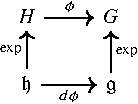
\includegraphics[height=1in]{exp-cd}
		\end{center}
	\else	
		\[
			\begin{tikzcd}
				H  \arrow[r,"\phi"] & G \\
				\mathfrak{h} \arrow[u,"\exp"] \arrow[r,"d\phi"'] & \mathfrak{g} \arrow[u,"\exp"'] 
			\end{tikzcd}
		\]
	\fi
\end{theorem}

\begin{proof}
	Let $X \in \mathfrak{h}$. Then $\gamma(t) := \phi(\exp(tX))$ is certainly a smooth curve in $G$ with 
	\[
		\gamma'(0) = \left. \frac{d}{dt} \right|_{t=0} (\phi \circ \exp)(tX) = d\phi(X). 
	\]
	Moreover, it's a one-parameter subgroup since $G$ is a homomorphism, so by uniqueness
	\[
		\gamma(t) = \exp(t d\phi(X))
	\]
	for all $t$, including $t=1$, which gives $\phi(\exp(X)) = \gamma(1) = \exp(d\phi(X))$, as desired.
\end{proof}

\begin{example}\label{ex:su2 to so3}
	As in \Cref{ex:exp on su2}, let $X=\begin{bmatrix} ix & y + iz \\ -y+iz & -ix \end{bmatrix} \in \mathfrak{su}(2)$. As we essentially showed in the proof of \Cref{prop:accidental isomorphisms}, the map $\psi \from \mathfrak{su}(2) \to \mathfrak{so}(3)$ defined by
	\[
		\psi\left(\begin{bmatrix} ix & y + iz \\ -y+iz & -ix \end{bmatrix}\right) := \begin{bmatrix} 0 & -2z & 2y \\ 2z & 0 & -2x \\ -2y & 2x & 0\end{bmatrix}
	\]
	is a Lie algebra homomorphism (in fact, isomorphism). Since $\SU(2)$ is simply-connected, \Cref{thm:Lie group Lie algebra correspondence} implies that there exists a Lie group homomorphism $\phi \from \SU(2) \to \SO(3)$ so that $\psi = d\phi$.
	
	By \Cref{thm:exp and homomorphisms}, we know that
	\[
		\phi(\exp(X)) = \exp(d\phi(X)) = \exp(\psi(X)).
	\]
	Since the image of $\phi$ is contained in $\SO(3)$, $\phi(\exp(X))$ acts on vectors $v \in \R^3$. By combining with \Cref{ex:general one-parameter subgroup of SO(3)}, we can see that $\phi(\exp(X))$ acts by rotating around the axis $v = (x,y,z)$ at double speed.
	
	In particular, if we assume $\|v\| =1$, then $\exp\left(\frac{\pi}{2} X \right)  \neq \exp\left(-\frac{\pi}{2} X \right)$ as elements of $\SU(2)$, but 
	\[
		\phi\left(\exp\left(\frac{\pi}{2} X \right)\right) = \phi\left(\exp\left(-\frac{\pi}{2} X \right)\right)
	\]
	as elements of $\SO(3)$ since the first rotates around axis $v$ by $\pi$ radians, and the second by $-\pi$ radians, which of course is the same rotation.
	
	This reflects the fact that the map $\phi\from \SU(2) \to \SO(3)$ is a double-covering.
\end{example}